\chapter{As the Sentence Unfolds: Oscillatory Dynamics of Language Processing in Verbally Competent Autistic Adults}
\label{ch:language_asc}

\begin{center}
    \large\textit{Abstract}
\end{center} 

{\abstractfont 
Autistic individuals often experience challenges and delays in language development, yet it remains unclear whether their language processing unfolds differently from that of neurotypical individuals in adulthood. In this study, we used EEG to examine real-time oscillatory neural dynamics as autistic adults and verbally and age-matched neurotypical controls read both structured sentences and pseudoword lists. Comparing these two conditions in reading revealed systematic spatiotemporal power dynamics across theta, alpha, beta, and gamma frequency bands across participants. These patterns included distinct lateralization dynamics in alpha and beta frequencies and a progressive intensification of beta oscillations as sentences unfolded, indicating cumulative processing of linguistic structure. Importantly, these oscillatory patterns appeared consistent across both autistic and neurotypical participants, with current analyses revealing no statistically significant differences in spatiotemporal progression or lateralization between groups. These findings suggest that sentence-level linguistic processing unfolds neurophysiologically in a similar manner in verbally competent autistic adults, suggesting that other underlying factors may contribute to language developmental delays in autism. \par
} 

\vspace{2cm}

\thispagestyle{empty}

\newpage

\section{Introduction}

Delays in language development are a common feature of autism, with approximately one-third of individuals remaining minimally verbal throughout their lives \citep{apa2013,kim2014,velikonja2019}. Although not a diagnostic criterion, autism is often first recognized due to atypical or delayed patterns of speech development during the second year of life, when most children of the same age begin to establish vocabularies comprising numerous words \citep{short1988}. However, such delays in expressive language during early preschool years are not unique to autism, and some individuals with autism acquire language typically despite marked social deficits \citep{anderson2007}. These observations underscore the complexity of language development in autism, highlighting the need to investigate whether language processing is fundamentally different, potentially involving distinct neural mechanisms even in verbally competent adults, or whether other underlying factors are responsible for the observed delays in language acquisition.

In search of a possible biomarker of autism and the associated language difficulties, a multitude of studies have been performed on the neural underpinnings of language processing in autism. Reduced neural activation to language and auditory stimuli has been found in brain regions typically involved in language \citep[for reviews]{groen2008,philip2012}. These results, however, are not always consistent \citep{tryfon2018}. A crucial challenge in interpreting these findings is that most studies depend primarily on neuroimaging techniques like fMRI, which restricts our insight into the neurophysiological processes involved in linguistic comprehension in autistic individuals. 

Electrophysiological investigations into language processing can provide insights on the mechanisms involved and their time course. These mechanisms operate at different frequencies that reflect circuit-level functions. These electrophysiological studies, however, are scarce in the current literature. A pair of studies investigated this in neurotypical individuals by having participants read sentences or pseudoword lists in an RSVP (Rapid Serial Visual Presentation) paradigm and applying Electroencephalography (EEG) and Magnetoencephalography \citep[MEG;][]{bastiaansen2010,bastiaansen2015}. This sentences vs. pseudoword list contrast probes the word-by-word operation of building a sentence-level representation, known as linguistic structure building. Firstly, they showed that higher power in the beta band was elicited at sensors over central, frontal, and bilateral parietal brain areas in response to linguistic structure building, as well as higher power in the theta band at sensors over right parietal areas. In terms of the time course of these effects, both studies found increasingly large beta and theta power differences between structure building and non-structure building conditions over the course of the sentence. Increases in beta and alpha power during linguistic structure building are suggested to reflect the maintenance of the sentence-level representation \citep{engel2010,lewis2016}, while theta may be linked to keeping sequentially ordered information in working memory \citep{roux2014,vignali2016}. In the gamma band, intracranial findings showed a ramping increase in power across the sentence structure \citep{fedorenko2016}, possibly reflecting (visual) information held in working memory \citep{bastos2018,honkanen2015,roux2014,vignali2016}. Whether these neural mechanisms are different in autistic individuals, is still an open question.

A more common finding for the neural basis of language processing in autistic individuals is reduced left-lateralized activation, often a consequence of increased involvement of the right hemisphere during language processing \citep{herringshaw2016}. This phenomenon was observed in semantic processing \citep{knaus2008}, lexico-semantic processing \citep{coffeycorina2008}, phonological processing \citep{dawson1986}, and sentence processing \citep{muller1999}. A recent, relatively well-powered study on linguistic structure building found reduced left-lateralization in autistic individuals using a similar linguistic structure building contrast as in the Bastiaansen et al. studies \citep{jouravlev2020}. Given the fact that most of these studies on the lateralization of language processing used fMRI, it is an unresolved question whether differences in lateralization in autism have a temporal component, i.e., whether they occur early or late during linguistic structure building. This research on lateralization is of clinical relevance because lateralization during language processing and measures of language ability are uniquely correlated in autistic individuals \citep{lindell2013}. Thus, findings could provide clues regarding the cause of autism-specific language difficulties. 

Considering the replicated findings in the two studies by Bastiaansen et al., the beta power increases provide a useful neural marker of structure building across the sentence. This marker can consequently be used to examine and compare structure building between autistic and neurotypical individuals, in addition to the degree of lateralization of structure building. Therefore, our aim for this study was to investigate the oscillatory activity during linguistic structure building, in particular the beta band, in autistic and neurotypical individuals. To tap into this broad linguistic process, we used the sentences vs. pseudoword list contrast from \cite{jouravlev2020}. First, higher beta power for sentences (linguistic structure building) compared to pseudoword lists was expected based on the findings from previous studies using this contrast \citep{bastiaansen2010,bastiaansen2015}, and this difference was expected to increase as the sentences unfold. Again based on previous work, we predicted that these effects would be maximal at electrodes over parietal regions. Given the inconsistent findings, we had slight expectations for stronger beta power in autistic individuals, although this is based on findings using different techniques and contrasts \citep{philip2012}. A second aim of our study was to investigate the degree of left-lateralization of power, in particular the beta band as an index of linguistic structure building, and its progression over time. This left-lateralization was calculated to compare between autistic and neurotypical individuals. Since one of the key motivations for using EEG was to observe potential temporal dynamics related to degree of lateralization in autistic vs neurotypical individuals, the beta power lateralization was computed and compared across time in one-second windows. Afterwards, these lateralization  indices were compared separately at each of these time points between autistic and neurotypical groups, and compared on their rate of linear increase or decrease. We expected beta power to be more left-lateralized in neurotypicals compared to autistic individuals, following the fMRI literature showing differences between the two groups. Moreover, this difference in lateralization of beta power between groups may reasonably be expected to be larger at later time points after there has ostensibly been more time for structure building to take place. By analyzing these oscillatory dynamics, we seek to determine whether linguistic structure building is altered in autism, shedding light on its potential role as a source of communicative variability in autistic individuals.

\section{Materials and methods}

\subsection{Participants}
Thirty-six autistic individuals (ASC) were included in this study on the basis of having a diagnosis of Autism Spectrum Disorder, as well as 40 neurotypical (NT) individuals. They were recruited from advertisements on social media, posters on campus, and Radboud University's participant database. They were included as autistic participants if they had an official diagnosis by a qualified clinician \citep{apa2013}, which was further validated by their scores on the Autism-Spectrum Quotient questionnaire \citep[AQ]{baron-cohen2001AQ}. The autistic participants can be classified as high-functioning given the low support demands in their daily lives. Exclusion criteria for all participants constituted severe cognitive impairment, systemic disease, a history of neurological impairment, and the use of psychotropic medication or systemic glucocorticoids. Each participant performed the experiment while EEG data was collected, after which the participants filled out a questionnaire with questions and tasks assessing a.o. their IQ, handedness, and autistic traits \citep{baron-cohen2001AQ,raven1989,veale2014}. Eight additional individuals participated in the study but their EEG data were not included in the study. The data of four of these participants were excluded due to technical malfunctions during the session. The other four participants' data were excluded due to poor data quality, for which less than 20 trials per condition were included after artifact rejection, or a full coverage of the head could not be established due to rejected bad electrodes. All participants gave written informed consent for the study protocol, which was approved by the local ethics committee (CMO region Arnhem-Nijmegen, file number 2019-6059). Participants were all compensated for their time investment and their travels.

The autistic and neurotypical individuals were matched on age, gender, handedness, and both verbal and non-verbal IQ (see Table~\ref{tab:ppt-stats-lang}). Statistical tests did not reveal differences between the autistic and neurotypical groups on gender balance (55.0\% vs. 44.4\% women, \textit{$\chi$\textsuperscript{2}} (1, \textit{N} = 76) = 0.48, \textit{p} = .49), on age (M \textpm{} SD 28.9 \textpm{} 6.8 vs. 27.0 \textpm{} 5.6, \textit{t}(74) = 1.29, \textit{p} = .20), on handedness (M \textpm{} SD 69.6 \textpm{} 69.8 vs. 84.7 \textpm{} 51.9, \textit{t}(74) = -1.15, \textit{p} = .25), or on verbal IQ measured by the Vocabulary and Similarities subscales of the Wechsler Adult Intelligence Scale \citep[128 \textpm{} 7 vs. 128 \textpm{} 16, \textit{t}(74) = -0.07, \textit{p} = .95]{wechsler1997} and performance IQ measured by the timed version of the Raven's Progressive Matrices test \citep[102 \textpm{} 9 vs. 103 \textpm{} 14, \textit{t}(74) = -0.35, \textit{p} = .73]{raven1989}. The Autism-Spectrum Quotient, as expected, showed a large difference between autistic and neurotypical participants (30 \textpm{} 9 vs. 14 \textpm{} 6, \textit{t}(74) = 9.23, \textit{p} <  .001), validating the distinction between the two groups.

\begin{table}[ht]
    \captionsetup{justification=raggedright, singlelinecheck=false, font = normal} % Left-align the caption
    \setlength{\tabcolsep}{12pt} % Adjust column spacing if needed
    \renewcommand{\arraystretch}{1.5} % Adjust row spacing
    \caption{Demographic data}
    \label{tab:ppt-stats-lang}
    \begin{tabular}{llll}
    \hline
    \textbf{} & \textit{ASC Group} & \textit{NT Group} & \textit{Group Difference} \\
    \hline
    N (women:men) & 40 (22:18) & 36 (16:20) & \textit{$\chi$\textsuperscript{2}}(1, N = 76) = 0.48, \textit{p} = .49 \\
    Age (years) & 28.9 (6.8) & 27.0 (5.6) & \textit{t}(74) = 1.29, \textit{p} = .20 \\
    Handedness (EHI) & 69.6 (69.8) & 84.7 (51.9) & \textit{t}(74) = -1.15, \textit{p} = .25 \\
    Verbal IQ (WAIS-III) & 128 (7) & 128 (16) & \textit{t}(74) = -0.07, \textit{p} = .95 \\
    Non-verbal IQ (RPM) & 102 (9) & 103 (14) & \textit{t}(74) = -0.35, \textit{p} = .73 \\
    Autism Quotient & 30 (9) & 14 (6) & \textit{t}(74) = 9.23, \textit{p} < .001 \\
    \hline
    \multicolumn{4}{l}{\small{Values are given as Mean (Standard Deviation). ASC, Autism Spectrum Condition; NT, Neurotypical.}} \\
    \end{tabular}
\end{table}

\subsection{Experimental design}
Neural responses to linguistic structure building were assessed with a reading paradigm based on \cite{fedorenko2010}, contrasting two conditions: sentences and pseudoword lists. Sequences in both conditions contained twelve words or pseudowords, presented serially at a rapid pace. The sentences and pseudoword lists were matched in the number of letters and syllables (letters: M\textsubscript{SEN} (SD\textsubscript{SEN}) = 72.5 (5.8), M\textsubscript{LIST} (SD\textsubscript{LIST}) = 72.6 (6.2); syllables: M\textsubscript{SEN} (SD\textsubscript{SEN}) = 20.7 (2.1), M\textsubscript{LIST} (SD\textsubscript{LIST}) = 20.8 (2.2)) and the topics described in the sentences were varied. The pseudoword lists were created by replacing the content words in the sentences with pseudowords, and scrambling all (function) words and pseudowords in the sentence. Two independent native Dutch raters confirmed that the pseudowords did not resemble existing Dutch words. To ensure that participants were closely reading all sequences, they were given a memory task to answer whether a probe word was presented in the sequence they just read. All sequences were presented in a randomized order for each participant, and presented in blocks of three sequences for each condition. Before each block, a fixation cross was presented for a random duration between 4000 and 7750 milliseconds. Before each sequence, a fixation cross was presented for 200 milliseconds. Each word or pseudoword was presented for 400 milliseconds. After the sequence, the memory probe word of the task was presented for 750 milliseconds. These durations are specified for the experiment presentation software, but the screen refresh time is added to these durations. For a subset of the participants in this study, the screen refresh times were 33 ms longer due to changes following hardware replacement. Importantly, the proportion of participants with different screen refresh durations is exactly the same between groups (75\% longer and 25\% shorter durations for both groups), ruling out the possibility of this difference explaining group effects. This difference is further corrected for in the data analysis section (see section \ref{preprocessing}). 

\begin{table}[ht]
    \captionsetup{justification=raggedright, singlelinecheck=false, font = normal} % Left-align the caption
    \renewcommand{\arraystretch}{1.5} % Adjust row spacing
    \caption{Example sequences for the two conditions with English translation.}
    \label{tab:example_sequences}
    \small
    \begin{tabular}{lp{12cm}}
    \hline
    \textit{Condition} & \textit{Example item} \\
    \hline
    SENT (sentence) & Meer dan duizend arbeiders werken in het moderne bedrijf tegenover het station. \\
     & \textit{More than a thousand employees work at the modern company across from the station.} \\
    LIST (pseudoword list) & van eingelzing bepen camzen parpisch uit naar groden kastren van naar moemels \\
     & \textit{from} eingelzing bepen camzen parpisch \textit{out to} groden kastren \textit{of to} moemels* \\
    \hline
    \multicolumn{2}{l}{\footnotesize *Only translations for existing Dutch function words.} \\
    \end{tabular}
    \normalsize
\end{table}

\begin{figure}[!ht]
	\centering
    \makebox[\textwidth][c]{\includegraphics[width=1\textwidth]{./Chapters/04_LanguageASC/Images/ExpDesign.eps}}
	\caption{Schematic of the task performed by autistic and neurotypical participants during the EEG experiment to ensure a close reading of the sequences. Sentences (shown here) or pseudoword lists were presented by showing every word or pseudoword consecutively for 400 ms, preceded by a fixation cross for 200 ms. After each sequence, participants were asked whether a target word (here: \textit{station}), on screen for 750 ms, was shown in the sequence they had just read, which they indicated via button press.}
    \vspace*{-10pt}
	\label{fig:exp-design}
\end{figure}




\subsection{Procedure}
Measurements took place in an electrically-shielded, sound-proof room. Before the EEG preparation started, participants were informed about the steps of the EEG preparation and measurement procedures. They received instructions about the task, including having to answer whether the probe word was part of the sequence that was presented before. They were instructed to use their left index finger to press a left button for yes and their right index finger to press a right button for no. They were also informed that while the reading and task decision tempo was quite high, their response would still be registered if they pressed the button after the probe word disappeared from the screen. Lastly, they were instructed to minimize head movement as much as possible during the task. The participants rested their head on a head and chin rest, reducing head movement, with a viewing distance of 59 cm. The words and pseudowords in the sequences and fixation crosses were presented in black text in the center of the screen with a light grey background. All text was presented in the Courier New font with size 18. Both the target word and `yes' and `no' were presented in red text. The measurement lasted for 12 minutes. 

\subsection{EEG recordings}
A fitting 64-electrode actiCap with active sensors was placed on participants' heads. The left mastoid electrode was used as a reference and an electrode at the center of the forehead as a ground electrode. To measure vertical eye movements, two electrodes were placed at the supra- and suborbital ridges of the right eye. For horizontal eye movements, two electrodes were positioned in a right-to-left outer canthal bipolar montage. Electrode impedance was kept below 25 kilo-ohms during the experiment. EEG data were amplified and collected with BrainAmp DC amplifiers at a sampling rate of 5000 Hz with a 0.1 - 1000 Hz band-pass filter. 

\subsection{Behavioral analysis}
To check whether participants were sufficiently engaged in the experiment, response rate for the memory task was calculated for each participant. With an independent \textit{t}-test (\textit{alpha} = 0.05) we assessed whether autistic and neurotypical individuals responded to a similar number of trials. Reaction time and accuracy to the memory task was recorded in order to compare the difficulty of the task between conditions and groups. To capture the variability in performance across trials and subjects, generalized linear mixed effects models in R (version 4.3.3) were used to investigate reaction time and accuracy with the \textit{lme4} package \citep{bates2015}. For modelling reaction time, participant group (autistic or neurotypical) and condition (sentence or pseudoword list) were included as fixed effects with their interaction term, together with a subject-specific intercept as random effect. This reaction time model was created to assume an inverse gaussian distribution with a log link function, optimized to only fit positive data \citep{lo2015}. The same model structure of fixed and random effects, but with a binomial distribution and a logit link function, was used to calculate effects for accuracy. Significance of the effects was identified with the \textit{lmerTest} package \citep{kuznetsova2017}, which uses Satterthwaite's method to calculate \textit{p}-values.

\subsection{EEG Preprocessing} \label{preprocessing}
EEG data were analyzed using the Fieldtrip toolbox \citep{oostenveld2011} in a MATLAB environment (R2020a; Mathworks, Inc.). The data were processed with a band-stop filter at 50, 100 and 150 Hz to reduce effects of power line noise (50 Hz). Artifact rejection was done in two stages of visual inspection of the data. First, the continuous EEG data were visually inspected for blinks, eye movements and high-frequency noise. Segments containing these artifacts were replaced with zeros. At trial definition, trials with less than two seconds of included data were excluded from further analyses. Afterwards, trials and channels containing noise and artifacts were rejected from the data on the basis of amplitude variance and kurtosis (all measured per trial across time). All scalp electrodes were re-referenced to the common average reference. Bad channels were repaired by reconstructing them from the average of their neighbouring channels. After artifact rejection, 19\% of all trials were excluded. Importantly, the number of rejected trials was comparable for the two conditions (M\textsubscript{SEN} = 19.2\%, M\textsubscript{LIST} = 17.8\%, \textit{t} (75) = 1.36, \textit{p} = .18) and the autistic and neurotypical groups (M\textsubscript{ASC} = 18.4\%, M\textsubscript{LIST} = 18.6\%, \textit{t} (75) = -0.09, \textit{p} = .93). Finally, all data were segmented from -300 ms to 5500 ms relative to the onset of the first word in the sequence. This trial duration was chosen as it corresponds to the shortest trial across all participants. Because of this procedure, the analysis excludes the last 396 ms of longer trial durations that are due to longer screen refresh times (12 (pseudo)words * 33 ms of screen refresh duration = 396 ms). This procedure was done to be able to include data from participants with both shorter and longer screen refresh times. Crucially, power changes in the sentence vs. pseudoword list contrast were not different for participants with short or long screen refresh times (see Supplementary Note \ref{suppl-note}).

\subsection{Sentences vs. pseudoword lists power and statistical analysis}
Time-frequency spectra were calculated for each trial separately using a sliding-window approach with a Hanning taper and the application of a fast Fourier transform. Frequencies were estimated between 2 and 100 Hz in steps of 2 Hz with a sliding window of 500 ms applied in steps of 20 ms. The sliding window length was chosen in order to optimize sensitivity in the beta band, the frequency band of interest, which tends to be relatively short-lived \citep{jones2016}. This means that the power in every time-frequency point represents a weighted average of -250 ms to 250 ms at the specified timepoint. Power values were then expressed as a relative change from the standard deviation of the power of all trials. This \textit{z}-scoring was done over all trials of both conditions within the full time window. This was performed separately for each channel, frequency, and time bin and resultant \textit{z}-scored power values were then averaged across trials. 

To calculate and compare power changes between the sentence and pseudoword list conditions, statistical testing was performed with cluster-based random permutation testing on power changes in the two conditions averaged over trials \citep{maris2007}. This method was chosen because it elegantly handles the multiple comparisons problem. Briefly summarized, for every data point (electrode-frequency-time point) a dependent \textit{t}-test is performed which generates uncorrected \textit{p}-values. These are compared against a pre-set significance level (here, 5\% two-tailed) and data points at which \textit{p}-values fall above this level are discarded. The remaining data is used to form clusters based on their adjacency in space (channels), frequency, and time. Cluster-level statistics are then computed by summing the \textit{t}-values of the data points that make up each cluster. Next, a permutation distribution is created by randomly assigning participant averages to one of the two conditions, an approach that is repeated 5000 times. Each permutation, cluster-level statistics are calculated, with the highest cluster-level statistic included in the permutation distribution. The cluster statistic for the measured data was compared against this distribution, and clusters that fell in the lowest or highest 2.5\% of the distribution were considered statistically significant. Statistical testing was first performed over the full frequency range between 2 and 100 Hz, allowing both spatial and spectral clustering for multiple comparison correction. Afterwards, the effects were separately tested in theta (3 - 7 Hz), alpha (7 - 13 Hz), beta (14 - 20 Hz) and gamma (60 - 80 Hz), averaged over the specific frequency band. The time window for which we tested the data was from 0 to 5200 ms relative to the onset of the first word of the sequences. Reported effect sizes for the cluster on the basis of which the H0 was rejected, were calculated by averaging over the data in this cluster. 

For a between-group comparison of power changes during linguistic structure building, the power difference between the sentence and pseudoword lists was calculated by subtracting the grand averages of the pseudoword lists condition from the sentences condition for each subject. Power changes were then compared between autistic and neurotypical individuals with cluster-based permutation testing using independent \textit{t}-tests (\textit{alpha} = 0.05). Bayes Factors were computed for between-group differences in power changes in peak channels and timepoints to assess the evidence for the null model and the model that specifies group.

To more sensitively assess whether this contrast, ostensibly designed to probe linguistic structure building, is constant or changes over time, a second test was performed.  For this test, a linear regression model across trial time course was fit to the power for each subject, condition and frequency band at its peak channel. These subject-specific regression fits were then compared between autistic and neurotypical individuals and sentence and pseudoword list conditions in an ANOVA with group, condition and their interaction as independent variables. 

\subsection{Laterality index}

For comparing lateralization of the linguistic structure building effect in the brain between groups and its progression over time, the previously calculated power values were split into five time windows of one second, spanning the trial time course, and averaged over these windows and over each of the four frequency bands. For these frequency bands and the five time windows, the difference in power between the sentence and pseudoword list conditions was calculated as the normalized power difference as the following: (SENT - LIST) / (SENT + LIST). This normalization was done to take into account electrodes that have differing levels of signal strength or quality. A laterality index for these power differences was calculated for all non-midline electrodes by subtracting the power of the right electrode from the power of the left electrode (Left - Right). This resulted in values representing the extent of the left-lateralization of the power difference for each electrode pair. While lateralization is more commonly calculated by dividing this Left-Right electrode difference by the sum of these two power values, this would lead to extreme values due to possible negative and positive values in the denominator. For this reason, we chose to exclude the denominator from the calculation. Note that these values represented the effects picked up on the scalp and not the precise location of the underlying neural generators due to volume conduction.

Grand averages of the laterality index were computed for each frequency band across time. To determine whether time-frequency power in the four frequency bands was lateralized in the first place, the laterality indices were compared to zero with the aforementioned cluster-based permutation method using dependent \textit{t}-tests (\textit{alpha} = 0.05). This was done for the autistic and neurotypical group separately. Crucially, the lateralization of power during linguistic structure building were then compared between the autistic and neurotypical participant groups with a cluster-based permutation method using independent \textit{t}-tests (\textit{alpha} = 0.05). The beta band was of particular interest in this analysis on account of previous studies showing it is the strongest index of linguistic structure building \citep{bastiaansen2010,bastiaansen2015}. 

To additionally assess group differences in language laterality more sensitively, we identified four electrodes where the sentence vs. pseudoword list contrast from the previous analysis was strongest across groups. These electrodes were therefore identified independently of the whole-brain laterality analysis. In these four peak electrodes, the average laterality index was calculated for each frequency band and time window. To determine whether power during linguistic structure building was lateralized in the first place, these average laterality indices were first compared against zero in both groups. This comparison was done with dependent \textit{t}-tests Bonferroni-corrected for the number of time windows (\textit{alpha} = 0.01). Afterwards, the laterality indices were compared between autistic and neurotypical participants with an independent \textit{t}-test (\textit{alpha} = 0.01), and Bayes Factors were computed and reported to assess the evidence for the null model or the model that specifies group status.

Finally, to statistically evaluate the time course of the laterality, a subject-specific linear regression model was fit to the laterality indices, mirroring the procedure for the power values. These regression fits were first compared against zero to determine whether lateralization in the four frequency bands varied over time. To investigate the difference in laterality time course for autistic and neurotypical individuals, the subject-specific regression fits on laterality values were subsequently compared in an independent \textit{t}-test (\textit{alpha} = 0.05). 

\section{Results}
\subsection{Behavioral task}
When asked if a word or pseudoword was part of a sentence or a list they read, responses were logged for 95.2\% of the trials on average (SD = 10.4\%), meaning participants did not respond to 4.8\% of the trials or responded too late. In addition, no participants responded to less than 50\% of trials and most participants (60\%) responding to all or all but one of the trials. These results indicate that participants attended to the task at hand. Response rates were within the same range for autistic and neurotypical individuals (M\textsubscript{ASC} = 94.2\%,  M\textsubscript{NT} = 96.5\%; \textit{t} (74) = -0.97, \textit{p} = .33), showing that the participant groups are similarly engaged with the task. In terms of analyzing response performance, we found that 82.5\% of trials were answered correctly on average (SD = 12.2\%). Much higher accuracy was found for responses for sentences than for pseudowords (M\textsubscript{SEN} = 89.8\%,  M\textsubscript{LIST} = 75.2\%; beta = 1.62, SE = 0.12, \textit{z} = 13.2, \textit{p} <  .001). A similar pattern was apparent for reaction times: participants took an average of 706 ms to respond (SD = 112.9 ms), but were much faster when responding to sentences than to pseudoword lists (M\textsubscript{SEN} = 657.9 ms,  M\textsubscript{LIST} = 754.1 ms; beta =  -0.13, SE = 0.01, \textit{t} = -17.7, \textit{p} <  .001). When comparing response measures between groups, we see that autistic and neurotypical individuals were equally accurate in task performance  (M\textsubscript{ASC} = 82.5\%,  M\textsubscript{NT} = 82.5\%; beta = -0.11, SE = 0.17, \textit{z} =-0.68, \textit{p} = .50). Yet, autistic people were overall slower to respond than neurotypical participants (M\textsubscript{ASC} = 733.8 ms,  M\textsubscript{NT} = 675.1 ms; beta = 0.09, SE = 0.04, \textit{t} = 2.07, \textit{p} = .038). No interaction between participant group and task condition was found either for accuracy (beta = -0.27, SE = 0.17, \textit{t} = -1.61, \textit{p} = .11) or reaction time (beta = -0.01, SE = 0.01, \textit{t} = -0.52, \textit{p} = .61), which suggests that autistic participants show an equally large linguistic task effect as neurotypical individuals.


\subsection{Time Frequency Analysis}
\subsubsection{Sentences vs. pseudoword lists across and between groups}
Cluster-based permutation analyses showed that time-frequency power when reading sentences was significantly higher than when reading pseudoword lists in the full frequency range from 2 to 100 Hz (\textit{p} <  .001, \textit{d} = 1.33). The difference in power was present in all channels and time points up to 46 Hz (see Fig~\ref{fig:tf-spectrum-full}a). Analyses focused on the four frequency bands individually confirmed this difference between conditions for the beta (\textit{p} <  .001, \textit{d} = 1.81), alpha (\textit{p} <  .001, \textit{d} = 2.99), theta (\textit{p} <  .001, \textit{d} = 2.27) and gamma (\textit{p} = .03, \textit{d} = 0.42) bands.

\begin{figure}[!ht]
	\centering
    \makebox[\textwidth][c]{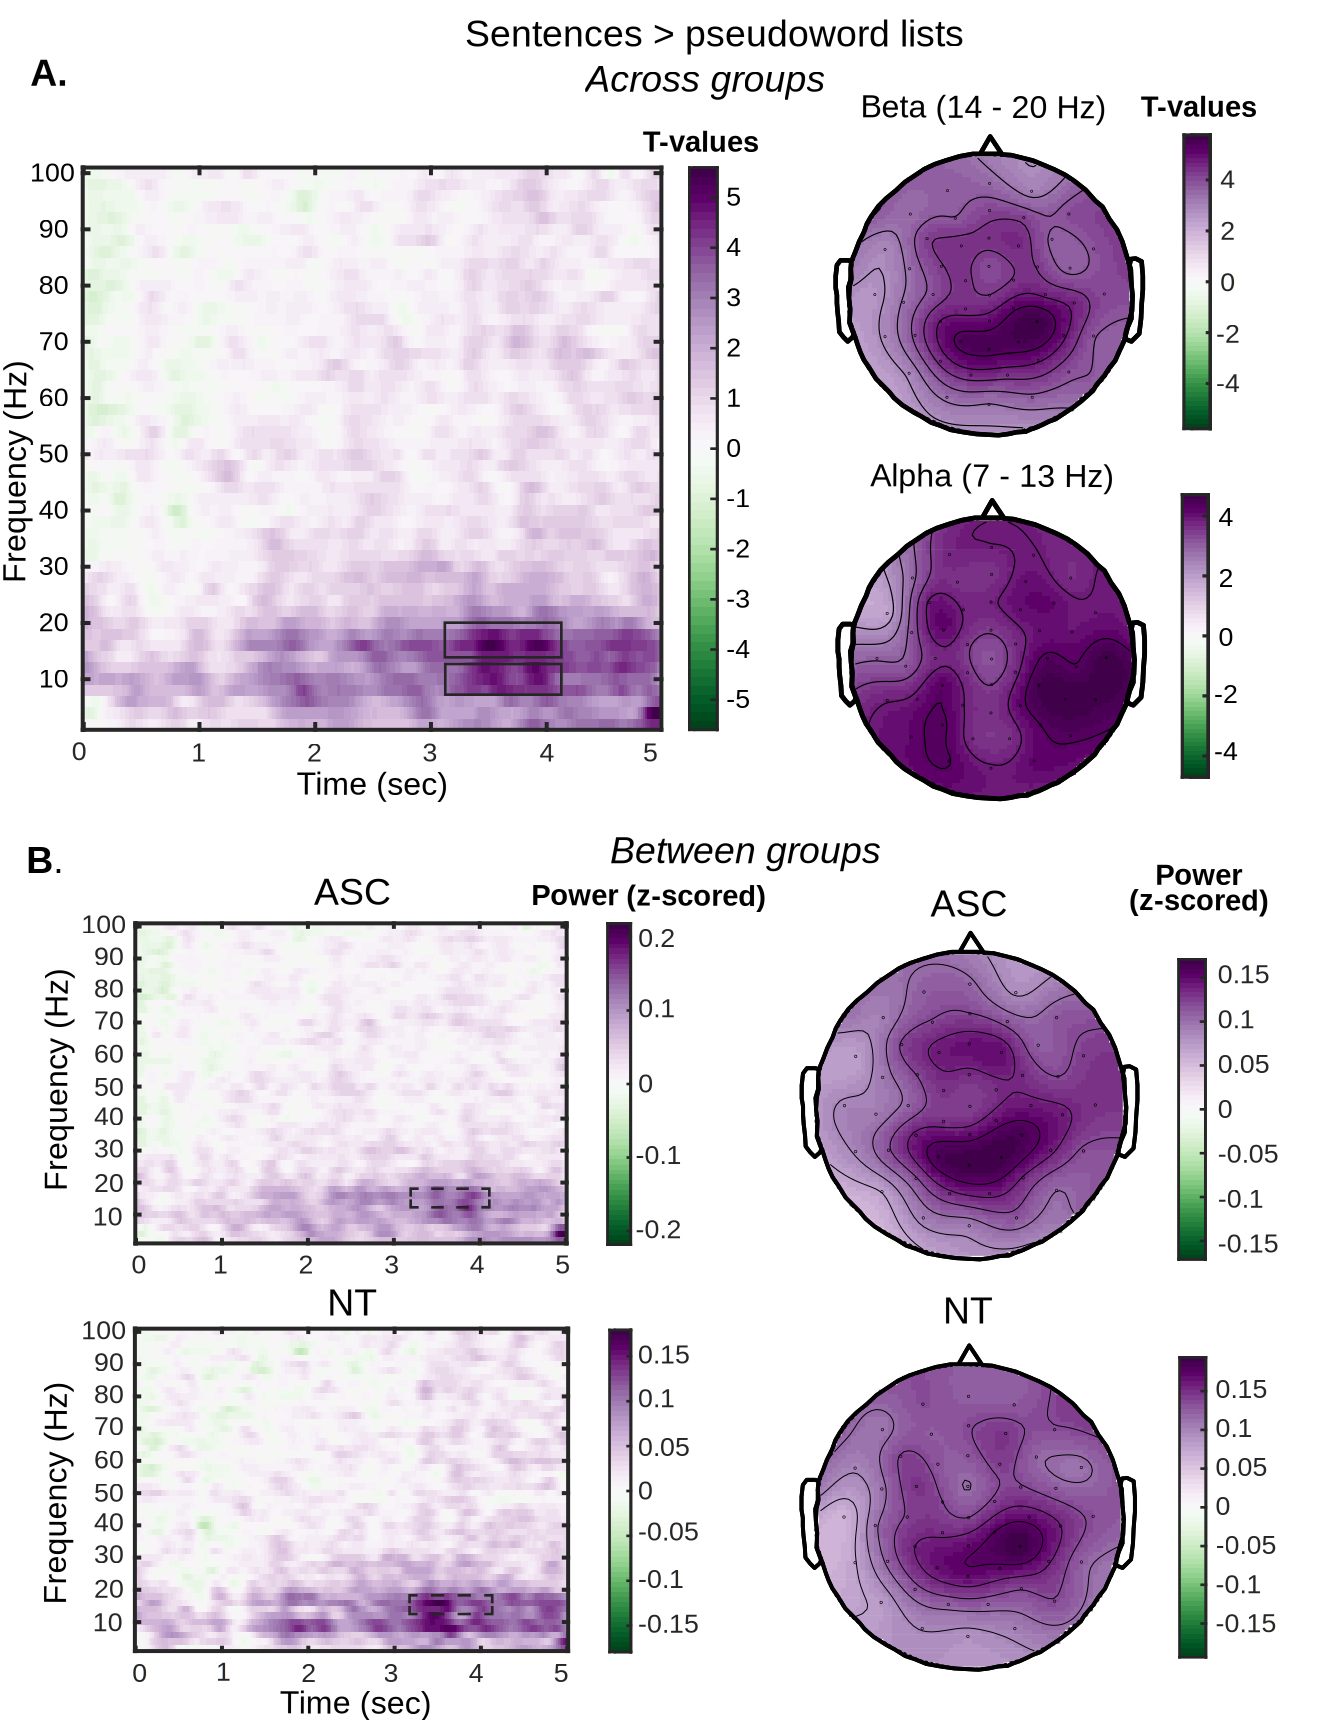
\includegraphics[width=.8\textwidth]{./Chapters/04_LanguageASC/Images/TFSpectrumFull_vert.eps}}
	\caption{Time-frequency (TF) dynamics in Sentences vs. pseudoword list contrast. (a) TF power is significantly different for the contrast, with power differences present across almost all channels, frequencies and timepoints. The color scale shows the relative difference in TF power (0 = no change). The timepoints and frequencies where the effect is strongest are indicated with boxes on the left, and the corresponding topography on the right for two different frequency bands: 14 - 20 Hz (beta) with bilateral posterior peaks, and 7 - 13 Hz (alpha) with a more widespread spatial effect. (b) TF power for the contrast was not different between neurotypical (NT) and autistic (ASC) participants. On the left, the similar TF spectra are shown, with the rectangle indicating the strongest power changes and on the right, the topography of this effect. }
    \vspace*{-10pt}
	\label{fig:tf-spectrum-full}
\end{figure}




The temporal dynamics of time-frequency power showed different patterns for the four frequency bands (see Fig~\ref{fig:tf-dynamics-topo}). The strongest power differences occurred in the latter part of the trial, peaking between 3 and 4 seconds after the onset of the first word, and in the beta band (around 16 Hz). This beta effect was primarily found at bilateral central posterior electrodes, peaking in the right hemisphere. Large power differences were also found for the alpha band (between 7 and 13 Hz), with a widespread spatial topography and strong effects at right parietal and left posterior electrodes. Given our experimental contrast, these alpha and beta differences likely contribute, at least partially and perhaps independently, to the cognitive process of linguistic structure building. 

\begin{figure}[!ht]
	\centering
    \makebox[\textwidth][c]{\includegraphics[width=1\textwidth]{./Chapters/04_LanguageASC/Images/TFDynamicsTopo.eps}}
	\caption{Time-frequency (TF) dynamics in Sentences vs. pseudoword list contrast across time and all participants for the theta (3 - 7 Hz), alpha (7 - 13 Hz), beta (14 - 20 Hz) and gamma (60 - 80 Hz) band.}
    \vspace*{-10pt}
	\label{fig:tf-dynamics-topo}
\end{figure}




Time-frequency power for this structure-building contrast was not significantly different between neurotypical and autistic individuals. The similar power spectra can be observed on the left hand side in Fig~\ref{fig:tf-spectrum-full}b, along with the topography of the strongest effect that was present in both groups. The similar time course of the two groups for both conditions can be seen in Fig~\ref{fig:tf-dynamics-peak}. A Bayesian analysis on the channels and timepoints showing maximal effects confirmed this lack of between-group differences for the beta (BF\textsubscript{NULL} = 3.31), alpha (BF\textsubscript{NULL} = 2.24), theta (BF\textsubscript{NULL} = 2.97) and gamma (BF\textsubscript{NULL} = 3.92) frequency bands. This indicates that oscillatory power in theta, alpha, beta, and gamma frequency bands during linguistic structure building are not different between neurotypical and autistic individuals. 

Subject-specific regression analyses indicated that progression of TF power over time was more positive while reading sentences compared to pseudoword lists in theta (\textit{d} = 0.48, \textit{p} = .004), alpha (\textit{d} = 0.46, \textit{p} = .005), and beta (\textit{d} = 0.96, \textit{p} <  .001; see Fig~\ref{fig:tf-dynamics-peak}a). This can be observed as the increasing difference in power over time between the conditions (see Fig~\ref{fig:tf-dynamics-peak}b). No significant difference between the condition in change over time was found for the gamma band (\textit{p} = .78). Time-frequency power change over time did not significantly differ for autistic and neurotypical participants in any of the four frequency bands, nor was there a significant interaction with condition. 

\begin{figure}[!ht]
    \vspace{10pt}
	\centering
    \makebox[\textwidth][c]{\includegraphics[width=.95\textwidth]{./Chapters/04_LanguageASC/Images/TFDynamicsPeak.eps}}
	\caption{Time-frequency (TF) power in the sentences and pseudoword lists (a) and difference of TF power between sentence and pseudoword list (b) across the trial time course for both groups. Power values are shown for the peak electrode in the sentences vs. pseudoword list contrast of the frequency band, of which the location is shown with scalp topography. Power differences over time between the two conditions were detected in the theta, alpha and beta band. No significant changes of TF power over time were found between autistic and neurotypical for any frequency band. Error bars indicate standard error. SENT = Sentences, LIST = Pseudoword lists. ** = \textit{p} < .001, * = \textit{p} < .01}
    \vspace*{-10pt}
	\label{fig:tf-dynamics-peak}
\end{figure}




\subsubsection{Lateralization of linguistic structure building}
Whole-scalp comparisons (all non-midline electrodes) were performed using cluster-based permutation statistics on the laterality indices of the sentences vs. pseudoword list contrast for the averaged one-second time windows and for the theta, alpha, beta, and gamma bands. Comparisons against zero in each participant group showed lower left-lateralization of power in the alpha band in the autistic individuals (\textit{p} = .002; see Fig~\ref{fig:laterality-topo}), driven by a cluster of frontal, lateral electrodes. No lateralized power was found in other frequency bands, nor in the neurotypical group. Despite this lateralization pattern in alpha, no differences in lateralization were found between autistic and neurotypical individuals in whole-brain comparisons for any of the four frequency bands. The similar lateralization patterns are shown across time in Fig~\ref{fig:laterality-dynamics-wholehem}.

\begin{figure}[!ht]
	\centering
    \makebox[\textwidth][c]{\includegraphics[width=1\textwidth]{./Chapters/04_LanguageASC/Images/LateralityTopo.eps}}
	\caption{Lateralization of time-frequency power in the sentences vs. pseudoword lists contrast detected across the hemisphere. Comparisons against zero showed significantly lower lateralization for autistic participants in the alpha band, driven by lateral electrodes. No significant changes of lateralization found between autistic and neurotypical for any frequency band. ** = \textit{p} < .01}
    \vspace*{5pt}
	\label{fig:laterality-topo}
\end{figure}




\vspace{.5cm}

\begin{figure}[!ht]
	\centering
    \makebox[\textwidth][c]{\includegraphics[width=.95\textwidth]{./Chapters/04_LanguageASC/Images/LateralityDynamicsWholeHem.eps}}
	\caption{Lateralization across the trial time course of time-frequency power in the sentences vs. pseudoword lists contrast for both groups averaged over the whole hemisphere. No significant changes of lateralization over time were found between autistic and neurotypical for any frequency band. Error bars indicate standard error. }
    \vspace*{-10pt}
	\label{fig:laterality-dynamics-wholehem}
\end{figure}


 

With a more spatially sensitive test, we inspected the topographies of the effects for the theta, alpha, beta, and gamma bands in the sentences vs. pseudoword list contrast, determined which electrodes showed maximal effects, and tested the laterality index between groups for these peak channels at each timepoint. For the beta, theta, and gamma band, independent \textit{t}-tests showed no statistically significant between-group differences in lateralization of the contrast at the selected electrodes in either of the five time windows (see Fig~\ref{fig:laterality-dynamics-peak}). This absence of group differences was corroborated by all Bayes factors for the null model being higher than for the model specifying group status (beta: BF\textsubscript{NULL} = 1.88 - 4.20, gamma: BF\textsubscript{NULL} = 2.63 - 4.13, theta: BF\textsubscript{NULL} = 1.82 - 4.13). For the alpha band, no significant between-group differences were found for four out of five timepoints (BF\textsubscript{NULL} = 2.39 - 4.19). There is evidence for a between-group difference in the alpha band between 1 and 2 seconds (BF\textsubscript{Group} = 1.4), although this difference did not pass the Bonferroni-corrected significance threshold (\textit{alpha}  = 0.01). These findings suggest that all frequency bands do not exhibit significant differential lateralization between neurotypical and autistic individuals during the process of linguistic structure building. 

After fitting a subject-specific linear regression model to the time course of lateralization during the sentence and pseudoword list conditions in the four peak channels, lateralization during linguistic structure building appeared stable across the trial, showing no deviating regression from zero (see Fig~\ref{fig:laterality-dynamics-peak}). Furthermore, lateralization was similarly stable for autistic and neurotypical individuals as no differences in time courses were found between the two groups. 

The analyses so far have regarded autistic and neurotypical individuals as separate categories, when autism can also be considered as a dimensional trait in the general population. To capture any lateralization effects beyond the case-control distinction of autistic and neurotypical individuals, we calculated Pearson's correlation between autistic trait strength and the sentences vs. pseudoword list contrast laterality indices for each time point at the four selected electrodes where the contrast was maximal in the analyses prior to computing the laterality index. Autistic trait strength was measured with participants' responses to the Autism-Spectrum Quotient questionnaire \citep[AQ;][]{baron-cohen2001AQ}. No statistically significant correlation was found for any of the four frequency bands. This corroborates the null finding in the case-control analysis that autism or autistic traits are not associated with lateralization differences during linguistic structure building. 

\section{Discussion}
While evidence on neurophysiological correlates of linguistic structure building during sentence reading in neurotypical individuals is growing, it remains unclear whether these are similar for autistic individuals. For this reason, we investigated how neural oscillations in autistic and neurotypical individuals are associated with linguistic structure building. Using a sentences vs. pseudoword list contrast, we replicated previous work showing that frequency-specific power associated with a sentences vs. pseudoword list reading contrast reaches maxima in the beta band (14 - 20 Hz) over bilateral parietal electrodes. The current study extended these findings with the novel result that this oscillatory activity during linguistic structure building is similar for neurotypical and autistic participants across theta, alpha, beta and gamma bands. We also observed larger differences over time during linguistic structure building in power in the beta, alpha, and theta bands but not the gamma band when comparing the regression fits over the course of the sequences. Furthermore, we showed that the degree of lateralization of power changes in the beta, alpha, theta and gamma bands associated with linguistic structure building was similar for neurotypical and autistic individuals. The degree of lateralization was similar at any time point in the sequence, and this stable degree of lateralization over time was present and similar in both groups. Crucially, taken together, these findings corroborate previous studies investigating frequency-specific beta power linked to structure building. In addition, the findings demonstrate that these beta effects, in addition to theta, alpha and gamma effects, are no different in autistic individuals. Moreover, they contradict fMRI findings \citep{jouravlev2020} showing differential lateralization in BOLD related to structure building between autistic and neurotypical individuals.

The peak effects of the linguistic structure building contrast were detected over bilateral parietal electrodes in the low-beta band, which is consistent with the location of large effects in earlier studies \citep{bastiaansen2010,bastiaansen2015}. Power in the beta band, in addition to the other frequency bands, was similar in our study for autistic and neurotypical individuals in this contrast. This deviates from findings in two fMRI studies who find lower activation for autistic individuals in left middle temporal gyrus during listening to sentences compared to rest \citep{muller1999}, and lower left inferior frontal activation but higher superior temporal activation when listening to sentences with the task to identify the agent or the patient in active or passive sentences \citep{just2004}. Notably, these fMRI contrasts and sentence processing tasks differ substantially from those of the current study, as well as the neuroimaging methods themselves. Since fMRI and EEG are not likely to capture the same neural signature, findings in one method are not expected to be identical to findings in the other method. Instead, they are complementary in capturing the underlying cognitive phenomenon.

The functional role of the beta power during linguistic structure building has previously been suggested to reflect syntactic unification, i.e., putting incoming words of a sentence together in a structure manner according to grammatical principles of the language to form a multi-word utterance \citep{bastiaansen2010,bastiaansen2015}. However, beta power has also been shown to decrease when syntactic unification becomes more demanding \citep{lewis2023}. Together with studies showing that beta power is also sensitive to other types of linguistic information during sentence comprehension (e.g., semantic and intonational anomalies), a more likely explanation might be that beta power supports the maintenance of a sentence-level representation during linguistic structure building \citep{lewis2016}. The maintenance role for the beta band in sentence comprehension is consistent with its role for other modalities such as motor control and visual attention \citep{engel2010}. This maintenance would be supported by increased top-down processing due to more prediction while processing a stimulus. This has been previously observed during visual attention and categorization tasks as increased beta power due to more top-down processing \citep{limanowski2020,antzoulatos2016}. These findings are consistent with our study, in which increased beta was observed for in the sentence reading condition. In this condition, a sentence-level representation could be formed, maintained and predicted for, which was not possible when reading pseudoword lists. 

While power in the gamma band is higher across sentences than pseudoword lists, we do not observe a power increase across the time course of the sequences when contrasting the two conditions. This finding differs from the results of an intracranial EEG experiment showing a ramping increase of beta power in a similar contrast over frontal and temporal electrodes \citep{fedorenko2016}. One potential explanation for this discrepancy is the difference in electrophysiological methods: it is possible that we did not pick up this ramping gamma effect due to the smearing of the signal from the volume conduction present in scalp EEG. Another possibility is that microsaccadic artifacts obscured a possible frontal effect in the current data, since those were not explicitly corrected for.   

A critical observation of the sentences vs. pseudoword list contrast that we used would be that it is a broad contrast which can capture a host of linguistic processes, not all of them related to structure building. The two conditions indeed differ in several respects, including lexical-semantics, syntactic structure, and situation model building. Yet, evidence that this contrast captures some linguistic structure comes from an ECoG study, in which the cognitive operation of merging words into multi-word phrases was probed with the same contrast \citep{nelson2017}. The authors successfully detected this `merge' operation, showing that the neural signal does not simply reflect the linearly increasing number of words, but responds to the demands of the syntactic tree-like structure of the sentence. Nonetheless, the primary goal of our study was not to probe the specificity of  the linguistic structure building captured by this contrast. We merely replicated existing findings linking this contrast to EEG, and investigated whether the neural marker of the process of interest is different for autistic and neurotypical individuals. 

In the current study, no lateralization differences were found in any frequency band between autistic and neurotypical individuals, contradicting the fMRI literature. This is likely due to the fact that fMRI and EEG do not capture the same neural signature, as previously mentioned. This also explains the fact that the laterality indices in the alpha and beta band of neurotypical participants were close to zero, indicating an absence of lateralization in the control group, and even negative lateralization across groups. This is in contrast with consistent left-lateralization of the BOLD signal in neurotypical individuals during language tasks \citep{fedorenko2010,pallier2011}. While gamma band power has previously shown correlations with the BOLD signal \citep{scheeringa2016}, left-lateralized gamma power was potentially obscured in our data by microsaccadic activity. Turning to research on lateralization of neural oscillations associated with language processing, we observe that the number of studies in this topic is scarce. Preliminary evidence on verb generation shows left-lateralization in region-of-interest analyses for beta oscillations (13 - 30 Hz) at inferior frontal electrodes and alpha oscillations (8 - 13 Hz) at superior temporal electrodes for neurotypical individuals \citep{nix2024}. Additional evidence using a phonological, orthographic and semantic task concerning short words found high-beta (21 - 28 Hz) oscillations showing a left-lateralized pattern across varying ages of neurotypical participants \citep{spironelli2010}. These studies, however, do not tap into the same linguistic process as in the current study, i.e. linguistic structure building, and can therefore not be directly compared with the current findings. For this reason, we had no strong expectations that the beta increase associated with linguistic structure building would be lateralized in the first place. Still, even with the absence of lateralization in neurotypical participants in our findings, one could have argued that a group difference can still exist through stronger right-hemispheric activity in autistic participants. This, however, was also not detected in our data. 

A straightforward possible explanation for the absence of lateralization differences between autistic and neurotypical individuals is the fact that fMRI and EEG have different spatial and temporal sensitivities. The lateralization differences and dynamics observed in \cite{jouravlev2020} and \cite{fedorenko2016} might be elicited from relatively localized neural activation, which could not be detected in our whole-brain analysis due to the mixture of neural sources we pick up at the electrodes. In our sensitive analysis which was focused on electrodes that showed the strongest contrast effects, we also observed no significant lateralization differences. But, as previously mentioned, there is no previous research on the lateralization in neurotypical individuals for this beta power increase during linguistic structure building, so we had no strong expectations that it would be lateralized. 

The high and similar levels of verbal IQ of the participant groups in this study raises the question of whether the autistic participants might be compensating by, for example, spending more attentional resources on the task, and whether this may explain the absence of lateralization differences. If the autistic participants were compensating in our study, then this was not reflected in our data as different oscillatory activity during linguistic structure building, nor in the laterality of that effect in comparison to neurotypical individuals. Instead, we have picked up neural markers of systems that function appropriately during linguistic structure building. Those systems might in turn be functioning appropriately because of compensatory mechanisms that we have not detected with our approach, but other studies that find group differences might have.

The null findings between groups across the analyses in this chapter may indicate a more general lack of behavioral, functional and structural brain differences between our autistic participants and control group. The participants included in this analysis, however, overlap for 63\% with the participants included in the analyses of chapter~\ref{ch:mentalizing_asc}, where we observe significant between-group differences in the fMRI data. In fact, the autistic participants of the current chapter overlap for 75\% with those in chapter~\ref{ch:mentalizing_asc}. This means that the vast majority of the autistic group of the current chapter can show significant neural differences from controls. Thus, the current null findings in the EEG analyses are more likely to be due to the experimental contrast than to a potentially inadequate group comparison.

The degree of lateralization of the beta power increase may have been expected to increase over time if the lateralization differences between autistic and neurotypical individuals was directly tied to linguistic structure building, because more structure building has presumably taken place when reading later parts of the sentences. Our findings however show that the laterality index for beta power is stable over the course of the sequences for the sentences vs pseudoword list contrast, and this stability over time is similar for the autistic and neurotypical participants. This absence of effects suggests that the lateralization of beta power linked to linguistic structure building during the task is not sensitive to increased structure building demands, and therefore likely does not tap into a compensatory process in autistic individuals. 

While existing evidence of reduced lateralization in language processing in autism is substantial \citep{lindell2013}, the findings in the current study suggest that beta power underlying linguistic structure building is not among the neural signatures that can be added to that body of evidence. One limitation of the methods used in this study, is the lack of spatial sensitivity of EEG. In future studies, source reconstruction methods could be used to try to better localize the neural generators that give rise to the scalp EEG effects. With this improved sensitivity, the findings might compare better to those from fMRI studies on lateralization in linguistic structure building \citep{jouravlev2020}.

Our preliminary findings suggest that sentence-level linguistic processing unfolds neurophysiologically in a similar manner in verbally competent autistic adults. While a more rigorous test involving source-level analyses would allow for a finer-grained understanding within normalized spatial frameworks, the current results begin to suggest that factors beyond sentence-level neural processing may contribute to the observed delays in language acquisition. This interpretation aligns with observations that, although the majority of individuals with autism ultimately acquire language, their social challenges often persist throughout life \citep{anderson2007}. Furthermore, several studies have reported that cognitive and neural processing in autistic individuals may be altered even in non-verbal social contexts \citep{mangnus2024bpcnni,wadge2019}. The ability to construct situated understanding in such contexts may play a crucial role in scaffolding the development of linguistic representations or computations. Once these linguistic mechanisms are acquired, they can be effectively engaged even outside social contexts, such as the experimental setting used in this study. The present findings suggest that this type of linguistic processing, when probed in isolation, may be fundamentally similar between autistic and neurotypical individuals. This raises the possibility that social and contextual dynamics, rather than intrinsic deficits in linguistic processing, might underlie the language developmental delays commonly observed in autism. 

To summarise, in our aim to compare the neural signatures of linguistic structure building between autistic and neurotypical individuals, we did not find such between-group differences in theta, alpha, beta or gamma bands, nor in their degree of lateralization. The absence of lateralization differences shows that the mantra of reduced language lateralization in autism does not necessarily apply to all facets of language processing or all neural measures linked to language processing. In general, our findings indicate that different aspects of communication rather than linguistic structure building might underlie the communicative difficulties observed in autism.


\newpage

\section{Supplementary information}

\subsection{S1: No difference in sentence vs. pseudoword list power changes for participants with shorter and longer durations} \label{suppl-note}
Baseline-corrected power changes in the sentence vs. pseudoword list contrast were compared between participants with shorter and longer screen refresh times to test whether this difference affected the EEG data. Power changes were first averaged over trials for both conditions, after which the power changes of pseudoword list trials were subtracted from those in sentence trials. These power differences were used in a cluster-based permutation test with the same parameters as described for the main sentence vs. pseudoword list contrast. No difference was found in the EEG contrast for participants with shorter and longer screen refresh times, indicating that this did not influence the results.

\subsection{S2: No significant group differences in lateralization of sentence vs. pseudoword list power in peak channels in any frequency band}

\vspace{-1cm}

\begin{figure}[!ht]
    \vspace{30pt}
	\centering
    \makebox[\textwidth][c]{\includegraphics[width=.95\textwidth]{./Chapters/04_LanguageASC/Images/LateralityDynamicsPeak.eps}}
	\caption{Lateralization across the trial time course of time-frequency power in the sentences vs. pseudoword lists contrast for both groups. Laterality indices are shown averaged over the four peak channels of the experimental contrast. The location of the channels is shown in the topography for each frequency band. No significant changes of lateralization over time were found between autistic and neurotypical for any frequency band. Additionally, no significant change of lateralization over time was detected in the linear regression fits. Error bars indicate standard error. }
    \vspace*{-10pt}
	\label{fig:laterality-dynamics-peak}
\end{figure}


 

\clearpage
